
\subsection{Creación de Planimetría}

% A- Módulo de planimetría
% - Objetivo del módulo	
Dentro del módulo de planimetría tenemos las herramientas necesarias para definir el escenario donde transcurrirán nuestras trayectorias. En primera instancia las trayectorias se definen a lo largo de un edificio, es por ello que las siguientes herramientas tiene el objetivo de caracterizarlo.   
% - Modelización 
%     - Diagrama de clases
%     - nodos, paredes, puertas, ascensores, escaleras, APs, plantas

Para la definición del escenario se ha definido clases en MATLAB que representarán los distintos objetos. La clase más grande que contiene a los demás elementos, es la clase \emph{building} (figura \ref{fig:esquemabuilding}). Estos objetos pueden contener objetos \emph{level} que representan las distintas plantas. A su vez, los objetos \emph{level}, contienen objetos type \emph{walls}, \emph{doors}, \emph{beacons}, \emph{stairs} y \emph{elevators}, de esta forma cada planta queda completamente definida. Estos objetos nos ayuda en la construcción de la trayectoria, ya que nos da las restricciones que debe seguir, además de dar información al modelo de simulación de trayectoria. También estan presentes en la generación de las señales, así como en el propio procesamiento de las señales. 

\begin{figure}[!ht]
    \centering
    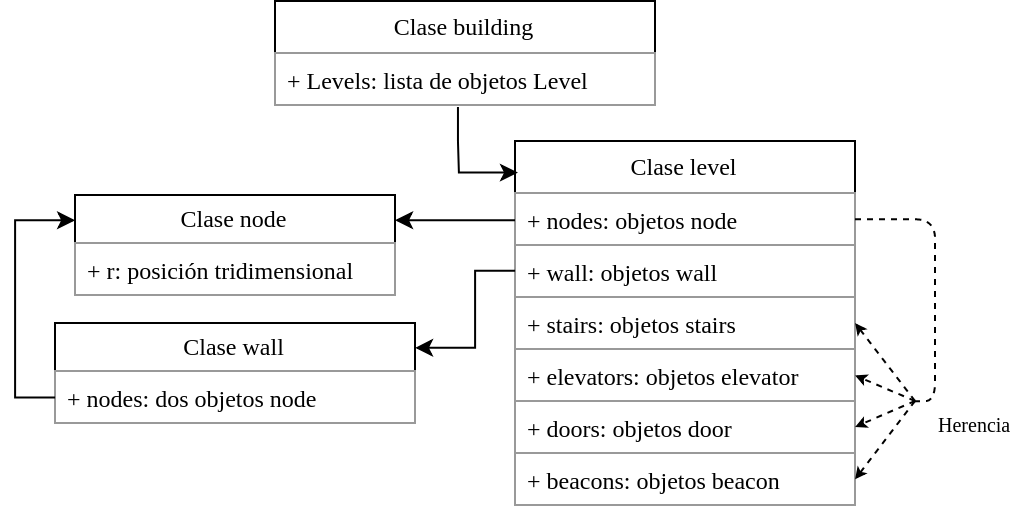
\includegraphics[width=1.0     \columnwidth]{img/Design/planimetria.png} 
    \caption[]{Esquema de la clase \emph{building}}
    \footnotesize
    \label{fig:esquemabuilding1}
\end{figure}

% - Explicación básica del proceso de generación de planimetría:  
%     - Clicks con el ratón
%     - mapa real como plantilla	 
Debido a que el proceso de creación de la planimetría puede ser tedioso, navindoor contiene una GUI capaz de generar un objeto \emph{building} (figura \ref{fig:interfaz1}). La interfaz nos permite crear los objectos antes mencionados con unos simples \emph{clicks}, además de permitir cargar una imagen de los planos reales con la que ayudarnos a construir la planimetría. 

% - Visualización 3D
Ademaś, cabe mencionar que la GUI contiene herramientas necesarias para la visualización en 3D, la modificación y eliminación de los elementos. De esta forma, la construcción de la planimetría es intuitiva.

\begin{figure}
    \centering
    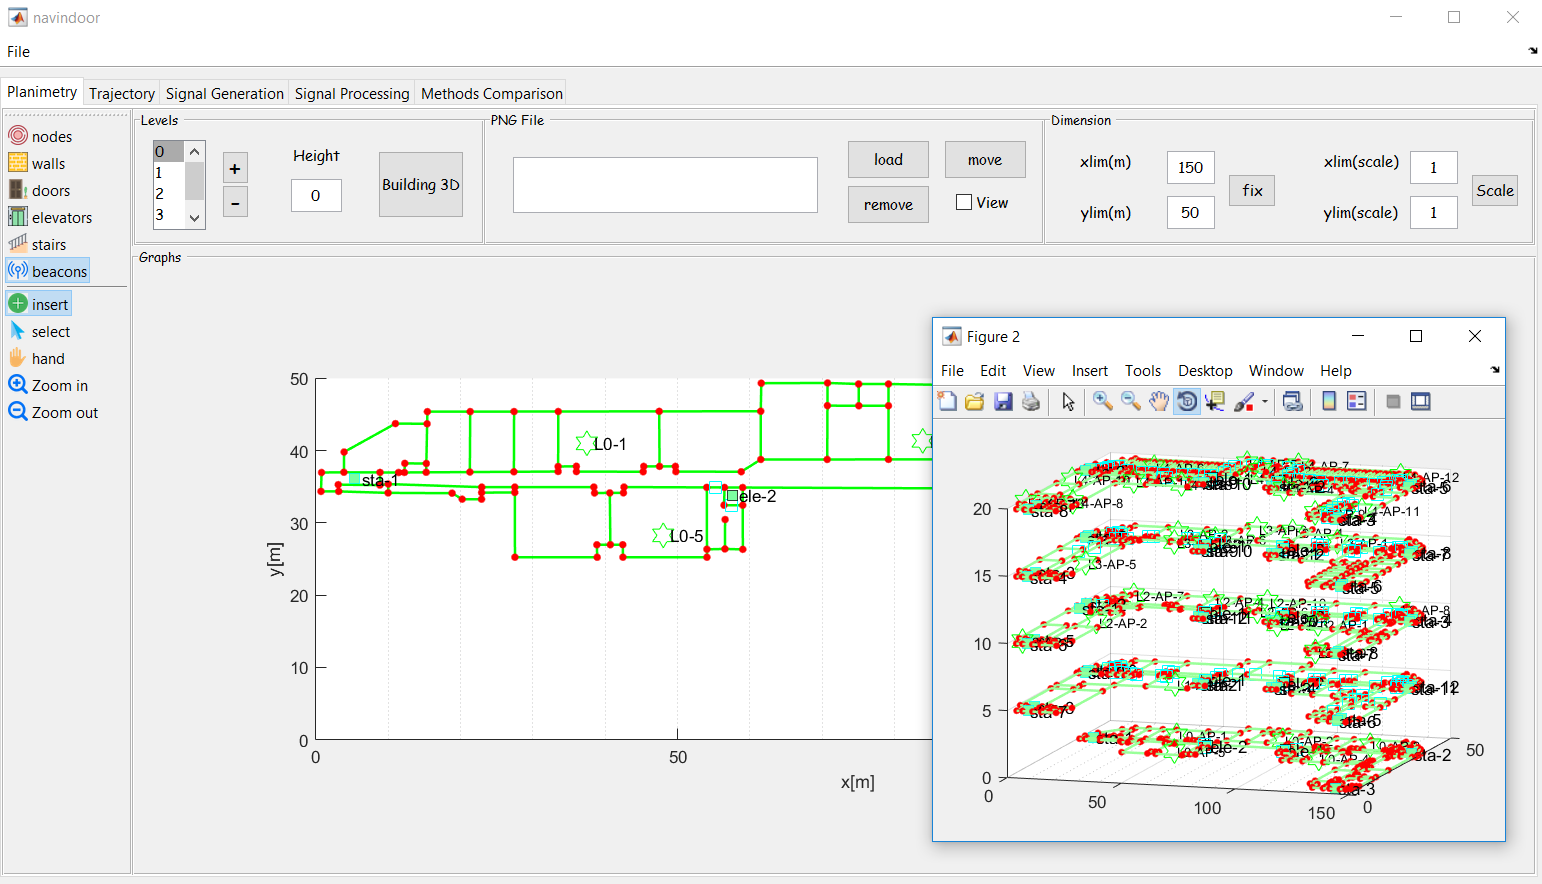
\includegraphics[width=0.8\columnwidth]{img/Design/1.PNG}
    \caption{Interfaz gráfica para el diseño de la planimetría \emph{building}.}
    \footnotesize
    En la imagen se muestra la interfaz con un edificio de cuatro plantas. La figura externa es una representación tridimensional del edificio.
    \label{fig:interfaz1}
\end{figure}

% Es improtante notar que la clase \emph{building} es una abstracción de la planimetría de un edificio, por lo que la traslación a otros formatos como \emph{XML} o \emph{JSON} es posible, y se están explorando por parte del equipo de desarrollo. Este desarrollo permitirá comunicaciones con plataformas como \emph{Open Street Maps}.






% ----------------------------------------------------------------------


